\section{Introduction}
\label{sec:introduction}

% Traditionally, DTs were conceived as virtual replicas used primarily for offline simulation, analysis, and optimization without continuous real-time interaction with their physical counterparts~\cite{grieves2014digital}.
% For example, early DT implementations in manufacturing enabled engineers to test and validate production processes virtually before deployment, thereby reducing downtime and costs~\cite{dt_industry_statoftheart}
With the widespread adoption of Internet of Things (IoT) and Industrial IoT (IIoT) technologies, Digital Twins (DTs) have evolved into \emph{active} components---i.e., software entities that maintain continuous bidirectional communication with their physical assets~\cite{grieves2014digital, dt_manufacturing_review, dt_industry_statoftheart}.
This paradigm shift allows DTs to provide dynamic digital representations updated through sensor data streams, supporting real-time monitoring, anomaly detection, and adaptive control~\cite{Cimino_2019}. 

In this context, integrating simulations into the DT architecture becomes increasingly critical.
Simulations would enable DTs to perform ``what-if'' analyses, optimize performance parameters, and validate control strategies before applying them to the physical asset~\cite{Boschert2016}.
The combination of real-time data and virtual experimentation allows DTs to anticipate issues and adapt to changing conditions in complex environments.
More in detail, we identified four primary motivations for integrating simulations into DTs:

\begin{figure*}[ht]
    \centering
    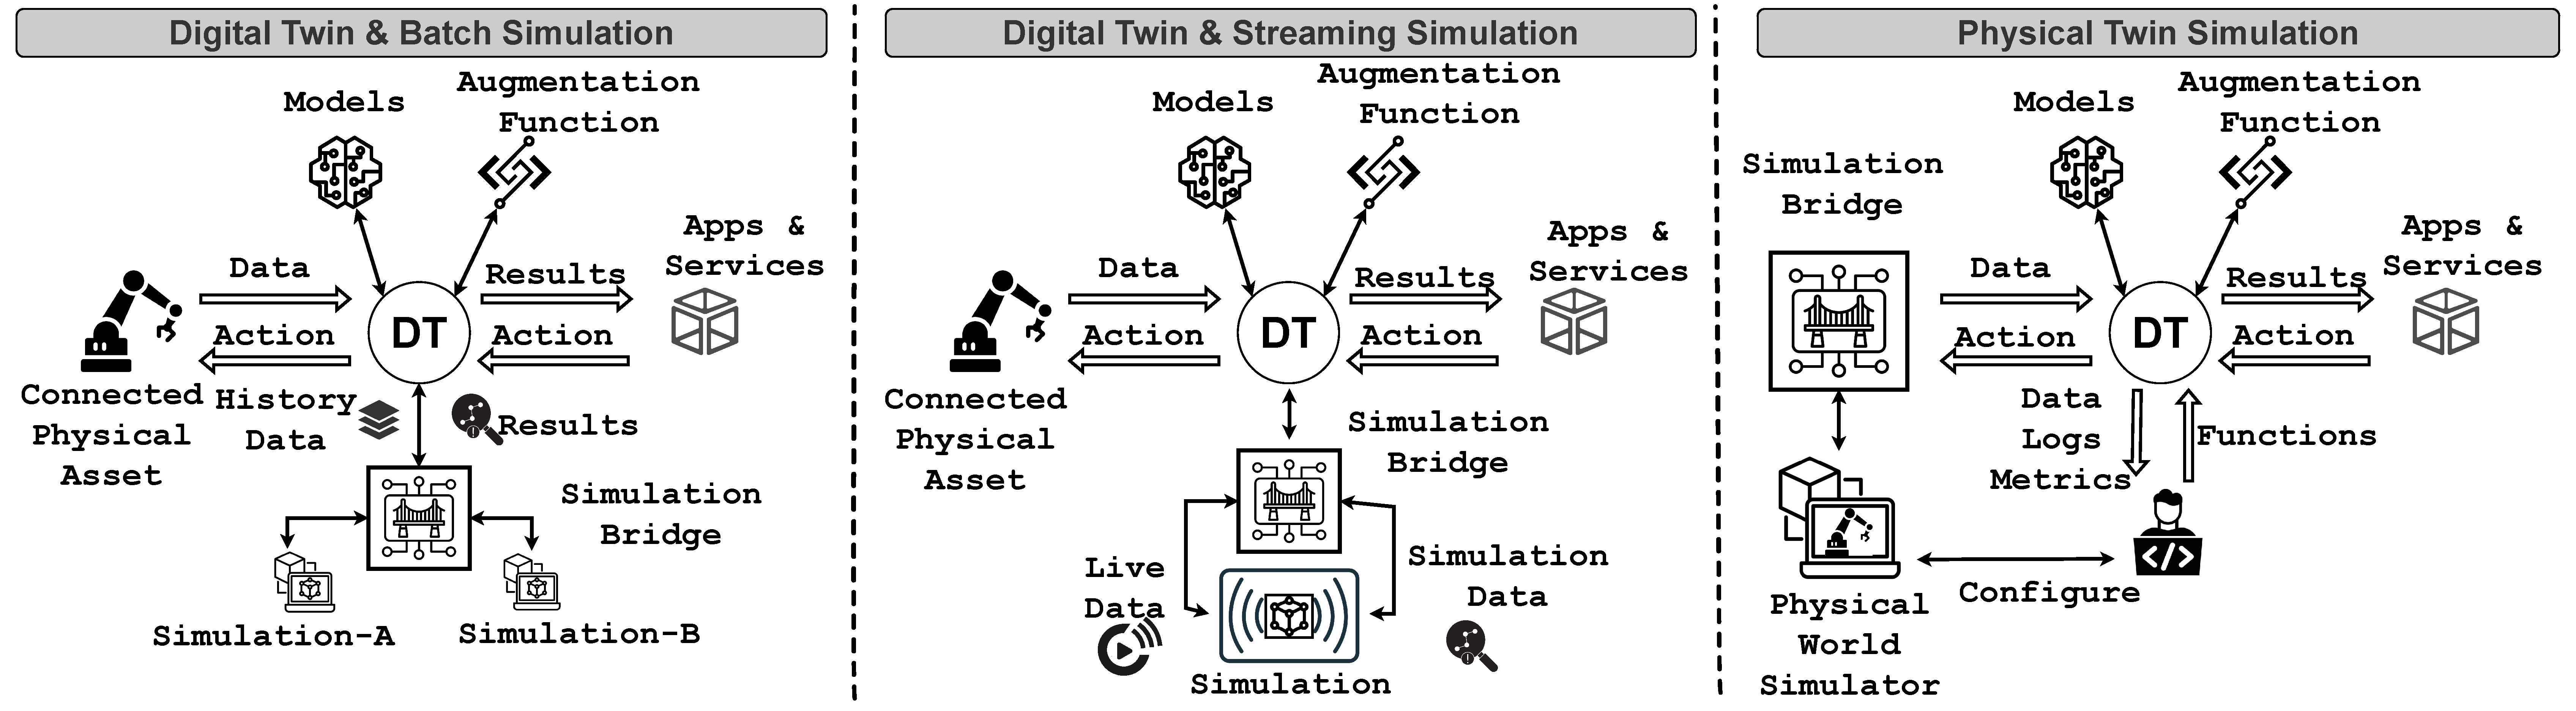
\includegraphics[width=\textwidth]{img/simulation_bridge_patterns.pdf}
    \caption{Overview of the Simulation Bridge enabling diverse interaction patterns between DTs and simulation environments.}
    \label{fig:dt_simulation_patterns}
    \vspace{-0.5cm}
\end{figure*}


\textit{(1) Enabling predictive and prescriptive capabilities.}  
While IoT-based DTs effectively capture the current state of physical systems through real-time data, open challenges remain in enhancing their ability to forecast future behavior and reason under uncertainty \cite{10015420}.
Simulation enhances DTs with predictive capabilities, supporting analysis under varying conditions such as equipment degradation, workload fluctuations, or environmental stressors~\cite{KLEIN2026103063}.
This shifts DTs from descriptive digital replicas to prescriptive and prognostic systems capable of anticipating outcomes and triggering proactive interventions.

\textit{(2) Coordinating heterogeneous simulations for complex systems.}  
Modeling complex systems often requires the orchestration of multiple, domain-specific simulations, each representing a different aspect of the physical system---e.g., mechanical dynamics, thermal effects, electrical behavior, or environmental interactions~\cite{10.1115/1.4049861,Fitzgerald2019}.
These simulations may operate at different time scales, resolutions, or levels of abstraction and must be integrated to ensure coherence and consistency. This is outside the scope of this paper.
%For example, a smart manufacturing DT might combine the kinematics of robotic arms with thermal simulations of material processing. 


\textit{(3) Supporting DT development in the absence of the Physical Twin (PT).}  
In many scenarios -- such as early-stage design, safety-critical applications, or high-cost manufacturing -- the physical system may not yet exist, be inaccessible, or pose operational risks.
In these cases, simulations -- e.g., of the IoT system~\cite{7568309} -- can act as surrogate PTs, generating mock behaviors and interaction patterns that allow the DT to be developed, tested, and validated in isolation~\cite{AITALLA20191331, 11087838}.

\textit{(4) Sharing simulation data across multiple DTs.}  
A single simulation model can serve multiple DTs, each potentially operating at different levels of abstraction and granularity.
For instance, a simulation of a production line may provide relevant data to DTs representing individual subsystems, such as robots or sensors, each requiring different views, resolutions, and update semantics. 

Despite these promising capabilities, the state of the art reflects only a partial integration of DTs and simulations~\cite{WOOLEY2023940}.
This paper presents the \emph{DT Simulation Bridge (DT-SB)}, a software framework designed to integrate DTs with multiple, heterogeneous simulation environments. The DT-SB enables bidirectional data exchange and supports diverse interaction patterns, allowing simulations to dynamically update the DT's internal state, while DTs can influence and tune simulation parameters in real time.

Unlike traditional co-simulation frameworks~\cite{Gomes&18}, the DT-SB connects a DT with multiple, independent simulations and acts solely as an intermediary. The coordination and aggregation of simulation results are delegated entirely to the DT, preserving architectural decoupling and maximizing flexibility.

We describe the modular architecture and core software components of the DT-SB, emphasizing its interoperability with diverse simulation models and protocols.

An experimental evaluation demonstrates the bridge’s effectiveness in accelerating iterative design cycles, facilitating virtual commissioning, and enabling live behavioral analysis under realistic operational conditions.


% The rest of the paper is organized as follows: Section~\ref{sec:relatedwork} reviews related work on DT–simulation integration, co-simulation, and distributed simulation frameworks. Section~\ref{sec:dt_sim_bridge} introduces the main interaction patterns supported by the DT-SB, highlighting their relevance across the DT lifecycle. Section~\ref{sec:sim_bridge_arch} presents the internal architecture of the DT-SB, detailing its modular components and communication mechanisms. Section~\ref{sec:sim-agents} describes the design and implementation of simulation agents, with particular focus on MATLAB and AnyLogic. Section~\ref{sec:experimental_evaluation} reports on the experimental evaluation of the DT-SB and its agents, analyzing latency and communication overhead. Finally, Section~\ref{sec:conclusion} summarizes the contributions and outlines directions for future work.
